\chapter{Analisis}
\label{chap:analisi}

%Analisis Aplikasi Sejenis
\section{Analisis Aplikasi Sejenis}
\label{lab:Analisis Aplikasi Sejenis}
% Aplikasi publik transport Android
\hspace{0.5cm} Aplikasi sejenis penulis temui bernama "Public Transport"\footnotemark[1]. Namun aplikasi tersebut hanya dapat dijalankan di sistem aplikasi android. Aplikasi "Public Transport" ini memanfaatkan Kiri API. Penggunaannya cukup sederhana. Di halaman awal pengguna dapat mengetikan lokasi awal dan tujuan. Selain dengan mengetik pengguna juga dapat menunjuk lokasi pada peta. Setelah lokasi dipilih sistem akan memastikan dengan memberi daftar nama jalan dan tempat terkait. Jika sudah memilih maka sistem akan mengeluarkan hasil pencarian rute.
\footnotetext[1]{\url{https://play.google.com/store/apps/details?id=travel.kiri.smarttransportapp}}

Berikut adalah tampilan dari aplikasi "Public Transport" (Gambar ~\ref{fig:home} sampai ~\ref{fig:peta}):

\begin{figure}[h]
	\centering
		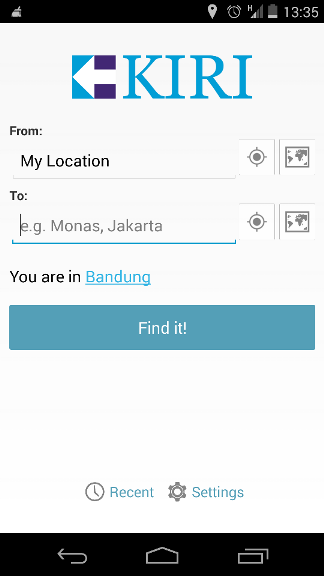
\includegraphics[scale=0.5]{Gambar/KIRI_Android/home}
	\caption{Tampilan awal aplikasi Public Transport}
	\label{fig:home}
\end{figure}

\begin{figure}[h]
	\centering
		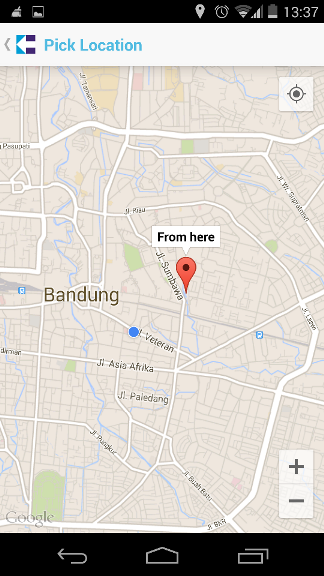
\includegraphics[scale=0.5]{Gambar/KIRI_Android/menunjuk_lokasi}
	\caption{Menunjuk lokasi pada peta}
	\label{fig:menunjuk}
\end{figure}

\begin{figure}[h]
	\centering
		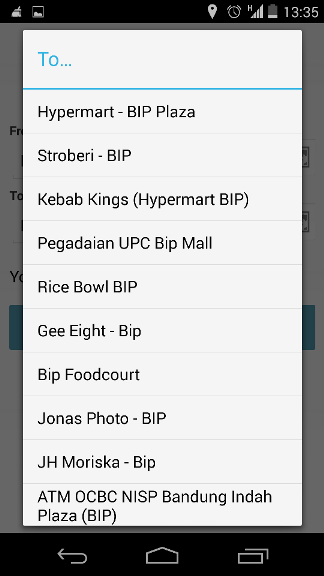
\includegraphics[scale=0.5]{Gambar/KIRI_Android/terkait}
	\caption{Memberikan daftar nama tempat dan nama jalan terkait}
	\label{fig:terkait}
\end{figure}

\begin{figure}[h]
	\centering
		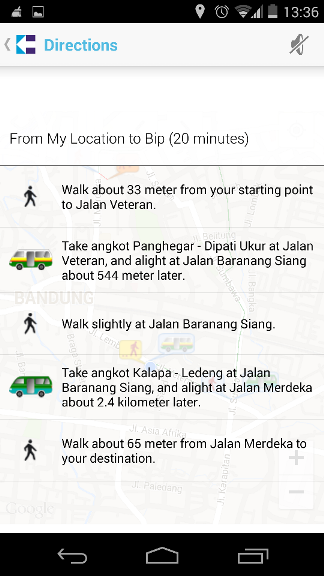
\includegraphics[scale=0.5]{Gambar/KIRI_Android/tampilan_daftar}
	\caption{Tampilan rute kendaraan umum dalam bentuk daftar}
	\label{fig:daftar}
\end{figure}

\begin{figure}[h]
	\centering
		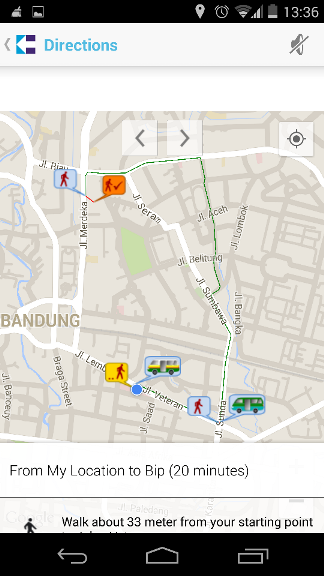
\includegraphics[scale=0.5]{Gambar/KIRI_Android/tampilan_peta}
	\caption{Tampilan rute kendaraan umum di peta}
	\label{fig:peta}
\end{figure}
% tampilannya, cara kerja, hal yang dapat dilakukan

\clearpage

%Analisis Analisis Program
\section{Analisis Aplikasi}
\label{lab:Analisis Aplikasi}
\hspace{0.5cm} Aplikasi akan dibuat mengguakan bahasa pemograman C\#. Aplikasi yang digunakan untuk membangun Aplikasi Pencari Rute Kendaraan Umum untuk Windows Phone adalah Visual Studio Express 2013. Pada sub bab ini akan dibahas diagram use case dan diagram kelas dari aplikasi yang akan dibangun. 

%Analisis Kebutuhan Aplikasi
\subsection{Kebutuhan Aplikasi}
\label{lab:Kebutuhan Aplikasi}
\hspace{0.5cm} Dari hasil observasi penulis dalam menentukan lokasi asal dan lokasi tujuan ada 2 cara. 2 cara tersebut yaitu dengan menulis alamat atau tempat dan dengan menunjuk pada peta. Cara menuliskan alamat atau tempat yaitu dengan menuliskan alamat atau tempat pada tempat yang disediakan untuk asal dan tujuan. Cara menunjuk pada peta yaitu dengan mengetuk layar di posisi yang diinginkan. Kedua hal tersebut pada dasarnya sama saja tetapi ada faktor kemudahan pengguna dalam pemakaiannya. Jadi penulis menyediakan 2 cara tersebut pada aplikasi yang penulis buat agar pengguna dapat memilih salah satunya.

\hspace{0.5cm} Pada saat menuliskan lokasi atau tempat atau menunjuk langsung pada peta mungkin saja terjadi kesalahan. Kesalahan tersebut bisa saja salah pengetikan atau nama tempat yang tidak ada. Maka dari itu dibutuhkan pemeriksaan terhadap masukan pengguna. Pemeriksaan tersebut dilakukan setelah pengguna memulai pencarian dengan menekan tombol "FIND".

\hspace{0.5cm} Untuk hasil keluaran ada 2 tipe seperti aplikasi peta lainnya. Kedua tipe tersebut adalah bentuk daftar dan bentuk peta. Bentuk daftar memudahkan dalam melihat tiap langkah rute. bentuk daftar memudahkan pengguna dalam melihat arah dan posisi lingkungan pada rute yang dipilih.

\hspace{0.5cm} Aplikasi yang penulis bangun didasarkan pada kebutuhan adalah sebagai berikut:
\begin{enumerate}
	\item Pengguna dapat memasukan lokasi asal dan lokasi tujuan pada bidang yang disediakan atau menunjuk langsung lokasi pada peta.
	\item Mendapatkan lokasi terkait menurut lokasi yang dimasukan pengguna.
	\item Menampilkan hasil rute angkutan umum dari lokasi asal ke lokasi tujuan.
\end{enumerate}

% SUB Analisis Kontrol yang Dipakai
\subsection{Analisis Kontrol yang Dipakai}
\label{lab:Analisis Kontrol yang Dipakai}
\hspace{0.5cm} Dari kebutuhan yang telah disebutkan diatas penulis menyadari pentingnya kontrol yang harus dipakai. Kontrol yang dimaksud termasuk tata letak, teks, pilihan, dan daftar. Kebutuhan akan kontrol penting bukan hanya untuk kebutuhan tapi memudahkan pengguna. 

\hspace{0.5cm} Untuk kontrol tata letak penulis membayangkan pengaturan yang tertata rapih dan beberapa elemen dalam satu baris atau kolom. Tetapi juga penulis tidak mengharapkan penggunaan kontrol tata letak yang rumit. Dari hasil pengamatan penulis kontrol tata letak yang cocok adalah Grid. Kontrol tata letak ini penulis pilih karena mudah diposisiskan sesuai baris dan kolom. Selain itu tampilan Grid akan menyesuaikan jika layar diputar dari posisi pemandangan ke posisi potret dan sebaliknya.

\hspace{0.5cm} Kontrol terhadap teks juga diperlukan untuk aplikasi ini. Kebutuhan yang diperlukan adalah mengeluarkan potongan teks yang dapat dibaca dan tempat pengguna memasukan teks. Untuk mengeluarkan teks yang dapat dilihat penulis akan menggunakan TextBlock. untuk masukan pengguna terhadap aplikasi penulis akan menyediakan TextBox sebagai tempat teks.

\hspace{0.5cm} Suatu aplikasi tentunya tidak hanya mempunyai satu halaman. Sama hal dengan aplikasi yang penulis buat memiliki beberapa halaman yang mempunyai tugas berbeda. Karena hal tersebut dibutuhkan kontrol untuk berpindah dari satu halaman ke halaman lain. Kontrol yang dibutuhkan yaitu kontrol tombol. Kontrol tombol akan mengeksekusi \textit{event click} yang memungkinkan indah halaman dan melakukan perintah.  

\hspace{0.5cm} Untuk menampilkan rute salah satu cara yang penulis lakukan adalah menampilkan dalam bentuk daftar. Bentuk daftar yang dapat dipakai di Windows Phone adalah menggunakan ListBox. ListBox akan menampilkan daftar rute satu per satu menurun ke bawah.

% SUB Analisis Terhadap Siklus Hidup Aplikasi
\subsection{Analisis Terhadap Siklus Hidup Aplikasi}
\label{lab:Analisis Terhadap Siklus Hidup Aplikasi}
\hspace{0.5cm} Aplikasi pada Windows Phone memiliki siklus hidup yang dijelaskan pada bab 2. Pengaturan aplikasi ini diatur sesuai konfigurasi awal sistem operasi Windows Phone. Tetapi pengaturan ini dapat diatur sesuai kebutuhan aplikasi. Karena di aplikasi ini terdapat keadaan yang berbeda dengan konfigurasi awal sistem operasi Windows Phone maka perlu adanya pengaturan ulang.

\hspace{0.5cm} Saat aplikasi dijalankan, pengguna memasukan lokasi asal dan lokasi tujuan dimasukan sampai pencarian rute dilakukan aplikasi akan berada di keadaan "Running". Tetapi ada kemungkinan pengguna berpindah aplikasi atau mematikan layar untuk menghemat daya maka aplikasi akan masuk ke keadaan "Suspended" dan setelah beberapa saat akan masuk ke keadaan "NotRunning". Jika dalam keadaan "Suspended" atau "NotRunnning" maka begitu aplikasi dibuka kembali keadaan aplikasi akan sama seperti keadaan terakhir sebelum keluar. Tetapi pada pemakaian oleh pengguna ada kemungkinan pengguna terlalu banyak mengakses aplikasi lain terlalu banyak dan mematikan layar terlalu lama maka aplikasi akan masuk ke keadaan "Close". Untuk menghindari hal pengguna mematikan layar terlalu lama maka keadaan "Supended" atau "NotRunning" harus diatur agar saat melihat peta dan mematikan layar aplikasi tidak masuk ke keadaan "Close". 

% SUB Analisis Peta
\subsection{Analisis Peta}
\label{lab:Analisis Peta}
\hspace{0.5cm} Untuk tampilan peta ada beberapa aspek yang perlu diperhatikan untuk memudahkan pengguna. Aspek yang perlu diperhatikan adalah tingkat zoom level, pandangan terhadap peta atau kartografi, dan mode warna. Setelah itu karena tampilan rute pada hasil pencarian dapat dimasukan gambar angkutan umum maka diperlukan penggunaan pushpin. Sesuai keluaran Kiri API yang mengeluarkan titik lokasi maka diperlukan teknik penggambaran rute yaitu menggunakan polyline.

\hspace{0.5cm} Tampilan awal peta di Windows Phone akan mengeluarkan peta dengan pandangan dunia. Karena aplikasi pencarian rute ini masih terbatas di Pulau Jawa, Indonesia terutama Jawa Barat maka zoom level harus diatur agar mengikuti lokasi pengguna dan di satu daerah saja. Jika pengguna berada di daerah Bandung maka zoom level pada peta disesuaikan pada daerah tersebut.

\hspace{0.5cm} Untuk cara pandang peta terdapat 4 pandangan yang disediakan Peta Windows Phone yaitu Road, Aerial, Hybrid, dan Terrain. Aplikasi ini adalah aplikasi pencari rute dan pandangan lebih banyak diarahkan ke jalan. Kebutuhan pengguna adalah nama jalan, kondisi jalan, dan kondisi sekitar. Untuk dasar pandangan tersebut pandangan yang penulis pilih untuk aplikasi ini adalah Road. Tambahan setelah mengatur pandangan peta yaitu mengatur warna dan penulis akan menggunakan mode warna terang sesuai bawaan.

%Kasih gambar road

\hspace{0.5cm} Untuk di setiap kota ada satu angkutan umum yang banyak dipakai yaitu angkutan kota(angkot). Namun bagi yang baru pertama mengunjungi suatu daerah dan mencari angkot mungkin akan kesulitan membaca trayek dari angkot tersebut. Namun ada satu cara yang mudah untuk membedakan angkot di setiap rute yaitu dari warna dan coraknya. Agar dapat memudahkan pengguna dan menghindari pengguna saat naik angkot maka Kiri API sudah menyediakan gambar angkot yang seusai dengan setiap rute. Gambar angkot tersebut akan ditepatkan di peta dengan suatu penampung beserta keterangan. Salah satu teknik untuk menempatkan gambar tersebut adalah dengan membuat lapisan terpisah di atas peta tempat gambar tersebut. Untuk hal tersebut penulis akan memanfaatkan Pushpin sebagai lapisan terpisah untuk menaruh gambar dan keterangan angkutan umum.

\hspace{0.5cm} Pencarian rute yang penulis gunakan untuk aplikasi yaitu dengan memakai Kiri API. Kiri API akan memberikan kembalian berupa titik-titik rute. Karena hal itu penulis harus menggambar rute tersebut sesuai jalan pada peta. Untuk hal tersebut penulis akan menggunakan Kelas Polyline pada Windows Phone untuk menggambarnya. Polyline yang digambar harus terlihat dengan jelas dan diberi warna yang kontras dengan warna peta.

% SUB Analisis Metode yang Dipakai
\subsection{Analisis Metode yang Dipakai}
\label{lab:Analisis Metode yang Dipakai}


%Analisis Diagram Use-Case dan Scenario
\subsection{Diagram Use-Case dan Scenario}
\label{lab:Diagram Use-Case dan Scenario}
\hspace{0.5cm} Diagram use-case adalah diagram yang menjelaskan interaksi sistem dengan lingkungan (contoh: pengguna). Berdasarkan analisa di atas maka pengguna dapat:
\begin{itemize}
	\item Mendapatkan lokasi pengguna berada.
	\item Memasukan lokasi asal.
	\item Memasukan lokasi lokasi tujuan.
	\item Menunjuk langsung lokasi asal dan tujuan pada peta.
	\item Memilih alamat atau tempat dari pilihan yang disediakan.
	\item Melihat rute kendaraan umum dalam bentuk titik dan \textit{pushpin} pada peta atau bentuk daftar dari tempat asal ke tempat tujuan.
\end{itemize}

Berikut adalah diaram use case saat pengguna mencari rute kendaraan umum (Gambar:~\ref{fig:UseCase}):
% Use case
\begin{figure}[h]
	\centering
		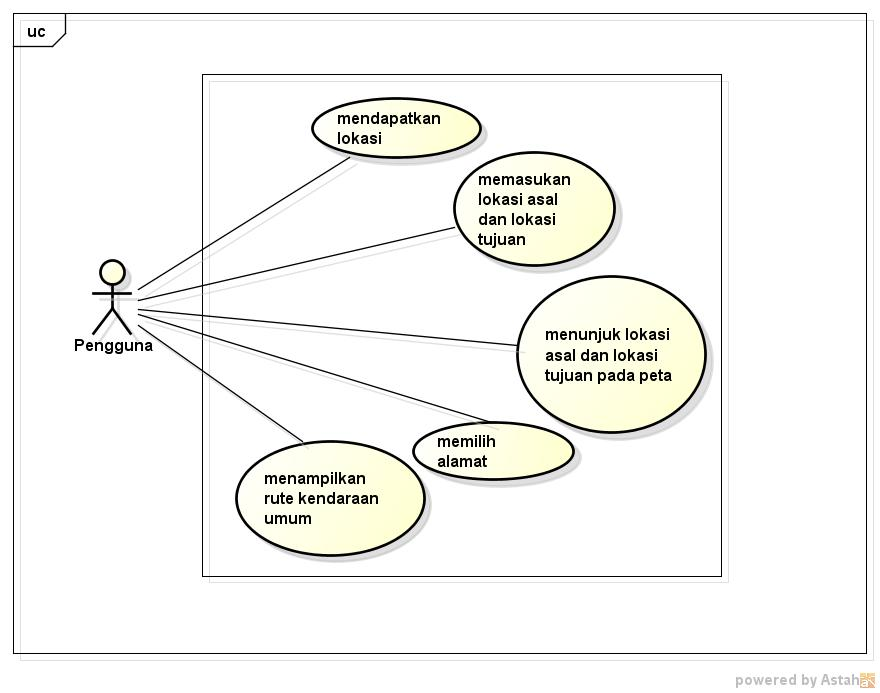
\includegraphics[scale=0.5]{Gambar/useCase_dan_Class/UseCase}
	\caption{Diagram Use Case}
	\label{fig:UseCase}
\end{figure}

% Skenario Melakukan pencarian rute 
\textbf{Skenario melakukan pencarian rute kendaraan umum}
Nama: Mencari rute kendaraan umum
Aktor: Pengguna
Kondisi Awal: Perangkat lunak dijalankan dan pengguna tidak tahu harus memakai kendaraan umum apa
Deskripsi: Pengguna memasukan lokasi awal dan lokasi tujuan
Kondisi akhir: Aplikasi memberitahukan kendaraan umum yang harus dinaiki pengguna.
Skenario:
\begin{enumerate}
	\item Pengguna memasukan lokasi awal dan tujuan atau menuntuk langsung pada peta.
	\item Sistem memberikan daftar tempat atau jalan terkait.
	\item Pengguna memilih dari daftar tempat atau jalan terkait.
	\item Sistem menentukan rute terbaik.
	\item Sistem menampilkan rute dalam 2 bentuk yaitu daftar dan titik pada peta.
\end{enumerate}
Eksepsi:
\begin{enumerate}
	\item Pengguna memasukan lokasi yang tidak terdaftar di sistem.
	\item Sistem memberi notifikasi bahwa lokasi tidak ditemukan.
\end{enumerate}

%Analisis Class Diagram
\subsection{Class Diagram}
\label{lab:Class Diagram}